%!Mode:: "TeX:UTF-8"
\documentclass[a4paper,12pts]{article}

%\usepackage[polish]{babel}
\usepackage{polski}
\usepackage[utf8]{inputenc}
\usepackage{fontspec}
\setmainfont{Calibri}

\linespread{1.15}

\usepackage{caption}
\captionsetup{%
	font={footnotesize},
	labelfont={bf}
}

\usepackage{anysize}
\usepackage{geometry}
\usepackage{multicol}
\usepackage{multirow}
\usepackage{graphicx}

% Plik szablonowy do wykorzystania pózniej - nie zmieniaj go!

\begin{document}
	\thispagestyle{empty}
	\begin{flushleft}
		Wydział Elektrotechniki, Automatyki, Informatyki i Inżynierii Biomedycznej \\
		Informatyka, rok II \\
		Zespół numer 3 \\
		Piotr Kucharski \\
		Dominik Zabłotny \\
		\vspace*{\fill}
		%-----------NUMER CWICZENIA--------%
		{\large \textbf{Sprawozdanie z ćwiczenia nr 51} } \\
		%-----------TEMAT ĆWICZENIA--------%
		Współczynnik załamania światła w ciałach stałych		
		\vfill	
		%-----------DATA-------------%
		15 listopada 2017r
	\end{flushleft}
	
	\newpage
	
	%---------------------------------------------------------------------------------------
	
		\section{Cel ćwiczenia}
	
	Celem wykonywanego ćwiczenia jest wyznaczenie współczynnika załamania światła dla szkła i zbadanie jego zmian w zależności od długości fali światła padającego.
	
	%--------------------------------------------------------------------------------------------------------------	
	
	\section{Wstęp teoretyczny}
	
	Światło padające na granice dwóch ośrodków ulega dwóm zjawiskom, odbiciu i załamaniu.
	
	\subsection{Prawo odbicia}
	
	Jeżeli światło pada na granicę dwóch ośrodków, to ulega zarówno odbiciu na powierzchni granicznej, jak i załamaniu przy przejściu do drugiego ośrodka tak, jak pokazano to na Rys. 1 dla powierzchni płaskiej.
	
	\begin{figure}[!h]
		\centering
		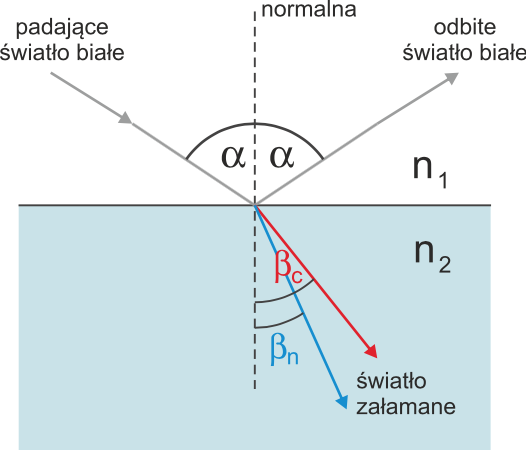
\includegraphics[scale=0.25]{odbicie.png}
		\caption{Schemat Prawa Odbicia \\ źródło: OPEN e-Podręczniki AGH - ,,Prawo odbicia i załamania"}
		\label{odbicie}
	\end{figure}
	
	\subsection{Prawo załamania}
	
	Prawo załamania (tzw. Prawo Snellius'a) definiuje stosunek sinusa kąta padania do sinusa kąta załamania, który jest równy stosunkowi bezwzględnego współczynnika załamania ośrodka pierwszego $n_1$, czyli współczynnikowi zględnego załamania światła ośrodka drugiego względem pierwszego. Kąty padania i załamania leżą w tej samej płaszczyźnie. Współczynnik załamania zależy od długości fali światła padającego. Po kilku przekształceniach trygonometrycznych otrzymujemy wzór:
	
	\begin{equation}
	\frac{sin\alpha}{sin\beta} = \frac{V_1}{V_2} = \frac{\lambda_1}{\lambda_2} = n = const
	\end{equation} 
	gdzie $\alpha$ to kąt padania, $\beta$ kąt załamanej wiązki światła, a n to współczynnik załamania światła ośrodka drugiego względem pierwszego.
	
	%--------------------------------------------------------------------------------------------------------------
	
	\newpage
	\section{Układ pomiarowy}
	
	Układ pomiarowy składa się z:
	
	\begin{itemize}
		\item Mikroskop wyposażony w czujnik mikrometryczny i nasadkę krzyżową,
		\item Śruba mikrometryczna,
		\item Zestaw płytek wykonanych z pleksiglasu oraz ze szkła, różnej długości.
	\end{itemize}
	
	%--------------------------------------------------------------------------------------------------------------
	
	\section{Wykonanie ćwiczenia}
	
	Schemat wykonania ćwiczenia:
	
	\begin{itemize}
		\item Wykonanie pomiaru grubości płytek wykonanych z pleksiglasu i szkła za pomocą śruby mikrometrycznej,
		\item Zamocowanie badanej płytki w uchwycie na stoliku mikroskopu,
		\item Odczyt wartości przesunięcia czujnika mikrometrycznego $a_g$,
		\item Wykonanie odczytów dla kolejnych płytek.
	\end{itemize}
	
	
	\section{Opracowanie wyników pomiarowych}
	\subsection{Dane pomiatrowe i wyniki}
	Dla poszczególnych próbek dokonano wielokrotnych pomiarów odległości płytki od obiektywu mikroskopu za pomocą śruby mikrometrycznej zamocowanej w mikroskopie gdy obraz powiększenia odpowiednio dla rysunku na górnej lub dolnej części płytki był wyraźny i ostry (zgodnie z uznaniem badających). Dane dla grubszej płytki pleksiglasowej zostały przedstawione w tabeli \ref{gruby_pleksi}.
	
	% Wstaw tabelę tutaj
	\begin{table}[!h]
		\centering
		\begin{tabular}{| c | c | c | c |}
			\hline
			\multicolumn{4}{|c|}{Materiał: pleksiglas}  \\ \hline
			\multicolumn{4}{|c|}{Grubość rzeczywista $d = 2.18$ [mm] } \\ \hline
			\multirow{2}{*}{lp.} & \multicolumn{2}{|c|}{Wskazanie czujnika} & Grubość pozorna \\ \cline{2-4}
			& $a_{\textrm{\footnotesize dolna}}$ [mm] & $a_{\textrm{\footnotesize górna}}$ [mm] & $h = a_{\textrm{\footnotesize dolna}} - a_{\textrm{\footnotesize górna}}$ [mm] \\ \hline
			1  & 4.83 & 3.35 & 1.48 \\ \hline
			2  & 4.80 & 3.35 & 1.45 \\ \hline
			3  & 4.84 & 3.36 & 1.48 \\ \hline
			4  & 4.82 & 3.37 & 1.45 \\ \hline
			5  & 4.81 & 3.35 & 1.46 \\ \hline
			6  & 4.76 & 3.28 & 1.48 \\ \hline
			7  & 4.72 & 3.31 & 1.41 \\ \hline
			8  & 4.73 & 3.30 & 1.43 \\ \hline
			9  & 4.79 & 3.31 & 1.48 \\ \hline
			10 & 4.77 & 3.32 & 1.45 \\ \hline
		\end{tabular}
		\caption{Wyniki pomiarów dla grubej płytki pleksiglasowej.}
		\label{gruby_pleksi}
	\end{table}
	\newpage
	Z pomiarów obliczono średnią arytmetyczną:
	\begin{equation}
		\Delta h_1 = \frac{\sum_{i = 1}^{10} h_{1_i}}{10} \approx 1.46 \textrm{ mm}
	\end{equation}
	którą następnie wykorzystano do obliczenia współczynnika załamania światła w pleksiglasie:
	\begin{equation}
		n_1 = \frac{d_1}{\Delta h_1} \approx 1.49
	\end{equation}
	
	Następnie zbadano płytkę pleksiglasową o mniejszej grubości. Celem badania tego samego materiału jest określenie wpływu grubości ciała na współczynnik załamania światła w ośrodku. Zmierzone dane zawarto w tabeli \ref{chudy_pleksi}.
	
	% Wstaw tabelę chudego pleksi tutaj
		\begin{table}[!h]
		\centering
		\begin{tabular}{| c | c | c | c |}
			\hline
			\multicolumn{4}{|c|}{Materiał: pleksiglas}  \\ \hline
			\multicolumn{4}{|c|}{Grubość rzeczywista $d = 4.93$ [mm] } \\ \hline
			\multirow{2}{*}{lp.} & \multicolumn{2}{|c|}{Wskazanie czujnika} & Grubość pozorna \\ \cline{2-4}
			& $a_{\textrm{\footnotesize dolna}}$ [mm] & $a_{\textrm{\footnotesize górna}}$ [mm] & $h = a_{\textrm{\footnotesize dolna}} - a_{\textrm{\footnotesize górna}}$ [mm] \\ \hline
			1  & 4.03 & 0.78 & 3.25 \\ \hline
			2  & 4.00 & 0.74 & 3.26 \\ \hline
			3  & 4.05 & 0.77 & 3.28 \\ \hline
			4  & 4.03 & 0.76 & 3.27 \\ \hline
			5  & 4.04 & 0.77 & 3.27 \\ \hline
			6  & 4.02 & 0.72 & 3.30 \\ \hline
			7  & 4.02 & 0.73 & 3.29 \\ \hline
			8  & 4.00 & 0.76 & 3.24 \\ \hline
		\end{tabular}
		\caption{Wyniki pomiarów dla cienkiej płytki pleksiglasowej.}
		\label{chudy_pleksi}
	\end{table}
	
	Analogicznie do grubej płytki pleksiglasu obliczony zostaje średni wynik: 
	\begin{equation}
		\Delta h_2 = \frac{\sum_{i = 1}^{8} h_{2_i}}{8} \approx 3.27 \textrm{ mm}
	\end{equation}
	oraz współczynnik załamania dla cienkiej płytki wykonanej z pleksiglasu:
		\begin{equation}
	n_2 = \frac{d_2}{\Delta h_2} \approx 1.51
	\end{equation}
	
	Aby porównać współczynnik załamania w innym ośrodku zbadano płytkę wykonaną ze szkła. Rodzaj szkła nie został określony, przez co pozostaje on nieznany. Zmierzone dane przedstawiono w tabeli \ref{szklo}.
	% Wstaw tabelę dla szkła
		\begin{table}[!h]
		\centering
		\begin{tabular}{| c | c | c | c |}
			\hline
			\multicolumn{4}{|c|}{Materiał: szkło nieznanego rodzaju}  \\ \hline
			\multicolumn{4}{|c|}{Grubość rzeczywista $d = 4.31$ [mm] } \\ \hline
			\multirow{2}{*}{lp.} & \multicolumn{2}{|c|}{Wskazanie czujnika} & Grubość pozorna \\ \cline{2-4}
			& $a_{\textrm{\footnotesize dolna}}$ [mm] & $a_{\textrm{\footnotesize górna}}$ [mm] & $h = a_{\textrm{\footnotesize dolna}} - a_{\textrm{\footnotesize górna}}$ [mm] \\ \hline
			1  & 4.31 & 1.77 & 2.54 \\ \hline
			2  & 4.30 & 1.79 & 2.51 \\ \hline
			3  & 4.29 & 1.80 & 2.49 \\ \hline
			4  & 4.29 & 1.79 & 2.50 \\ \hline
			5  & 4.31 & 1.79 & 2.52 \\ \hline
			6  & 4.31 & 1.79 & 2.52 \\ \hline
			7  & 4.30 & 1.80 & 2.50 \\ \hline
			8  & 4.30 & 1.80 & 2.50 \\ \hline
		\end{tabular}
		\caption{Wyniki pomiarów dla płytki szklanej nieznanego rodzaju.}
		\label{szklo}
	\end{table}

	Z uzyskanych danych obliczono średnią grubość pozorną:
	\begin{equation}
		\Delta h_3 = \frac{\sum_{i = 1}^{8} h_{3_i}}{8} \approx 2.51 \textrm{ mm}
	\end{equation}
	co pozwala na obliczenie współczynnika załamania światła dla szkła:
	\begin{equation}
		n_3 = \frac{d_3}{\Delta h_3} \approx 1.72
	\end{equation}
		
	\subsection{Niepewność pomiarowa}
	Niedokładność pomiaru grubości rzeczywistej badanej płytki jest niepewnością typu B, ponieważ nie jest możliwe określenie błędu na podstawie wielokrotnych pomiaów. Jest ona równa niepewności podanej przez producenta na tabliczce znamionowej śruby mikrometrycznej:
	\begin{equation}
		u(d) = 0.01 \textrm{ mm}
	\end{equation}
	
	Analogicznie dla pomiaru odległości płytki od obiektywu mikroskopu - śruba mikrometryczna zamocowana na mikroskopie posiada niepewność ustaloną przez producenta, stąd:
	\begin{equation}
		u(a) = 0.01 \textrm{ mm}
	\end{equation}
	
	Błąd wyznaczenia średniej grubości pozornej badanych płytek jest niepewnością typu A, którą wyrażamy estymatorem odchylenia standardowego dla $k$ prób:
	\begin{equation}
		u(h) = \sqrt{\frac{1}{k}\sum_{i=1}^{k}(\Delta h - h_i)^2}
	\end{equation}
	Błędy dla poszczególnych pomiarów zostały wyrażone w tabeli \ref{niepewność_h}.
	\begin{table}[!h]
		\centering
		\begin{tabular}{|c|c|}
			\hline
			Rodzaj materiału  &  Niepewność pomiarowa $u(h)$ [mm] \\ \hline
			Gruby pleksiglas   &  0.024 \\ \hline
			Cienki pleksiglas  &  0.020 \\ \hline
			Szkło nieznanego rodzaju & 0.016 \\ \hline
		\end{tabular}
		\caption{Niepewności pomiarowe średniej grubości pozornej}
		\label{niepewność_h}
	\end{table}

	Niepewność wyznaczenia współczynnika załamania światła jest niepewnością złożoną zależną od niepewności pomiaru rzeczywistej grubości oraz błędu średniej grubości pozornej. Wyraża się ją wzorem:
	\begin{equation}
		u(n) = \sqrt{\left(\frac{\delta n }{\delta d} u(d) \right)^2 + \left(\frac{\delta n}{\delta h} u(h)\right)^2} = \sqrt{\left(\frac{1}{h}u(d)\right)^2 + \left(-\frac{d}{h^2}u(h)\right)^2}
	\end{equation}
	Wyniki zostały przedstawione w tabeli \ref{niepewność_n}
	\begin{table}[!h]
		\centering
		\begin{tabular}{|c|c|}
			\hline
			Rodzaj materiału & Niepewność pomiarowa $u(n)$ \\ \hline
			Gruby pleksiglas & 0.025 \\ \hline
			Cienki pleksiglas & 0.0097 \\ \hline
			Szkło nieznanego rodzaju & 0.012 \\ \hline
		\end{tabular}
		\caption{Niepewność obliczenia współczynnika załamania światła}
		\label{niepewność_n}
	\end{table}

	\section{Podsumowanie wyników}
	Końcowe wartości wpółczynnika załamania światła zostały zestawione w tabeli \ref{podsumowanie_wynikow}.
	\begin{table}[!h]
		\centering
		\begin{tabular}{|c|c|c|c|}
			\hline
			Rodzaj materiału & Wartość tabelaryczna & Wartość obliczona & Zgodność z wynikiem tabelarycznym \\ \hline
			Gruby pleksiglas & 1.489 & 1.49 $\pm$ 0.025 & TAK \\ \hline
			Cienki pleksiglas & 1.489 & 1.51 $\pm$ 0.0097 & NIE \\ \hline
			Szkło nieznanego rodzaju & 1.4 - 1.9 & 1.72 $\pm$ 0.012 & TAK \\ \hline
		\end{tabular}
	\caption{Podsumowanie wyników oraz porównanie z wartościami tabelarycznymi}
	\label{podsumowanie_wynikow}
	\end{table}

	\section{Wnioski}
	Jedynym wynikiem nie zawierającym się w granicach niepewności podstawowej i rozszerzonej jest współczynnik załamania dla cienkiego pleksiglasu. Jest to spowodowane nie idealnym określeniem czy obraz powiększenia jest już dostatecznie ostry (niedokładność ludzkiego oka oraz niedoskonałość wyświetlacza mikroskopu) oraz możliwą wadliwością wyświetlacza wyniku śruby mikrometrycznej mikroskopu. Podczas delikatnej regulacji położenia stolika z badanym ciałem względem obiektywu w odległościach mniejszych niż 1 mm  od mikroskopu wskazówka śruby mikrometrycznej nie wychylała się, po czym gwałtownie zmieniała swoje położenie do dalszego obszaru, jednak nie wiadomo z jaką precyzją, co zwiększa niedokładność pomiarów dla cienkiej płytki pleksiglasu. Jednakże, wynik ten w granicach niepewności rozszerzonej zgadza się z współczynnikiem załamania światła dla grubszej płytki wykonanej z pleksiglasu, przez co wnioskujemy, że wartosć współczynnika załamania światła nie zależy od grubości materiału.
	
\end{document}